\section{Deep Recurrent Attentive Writer}\label{sec:draw}

One of the central challenges of the ELBO as presented in equation \ref{eq:elbo} is that the probability of a pixel in the output being activated is not conditional on whether the pixels surrounding it has is activated. This means that the entire canvas is conditioned on a single sample. The Deep Recurrent Attentive Writer (DRAW) aims to solve this problem by creating an iterative algorithm updates parts of, or the whole canvass, multiple times (\cite{Gregor2015}). In this thesis we make three central modifications to the algorithm. 

\begin{itemize}
\item Originally DRAW views parts of the input conditioning the latent sample $\mathbf{z_t}$ on differently sized patches of the input image. We modify the model such that the model gets glimpses of the same size at each time step. This is done to make samples comparable between time steps in line with the work of \citet{Harris2019}
\item The attentive part of DRAW as described by \citet{Gregor2015} is a set of Gaussian filters that pick out a part of the input allowing the image to focus on discrete regions. We modify the algorithm to allow the use of a convolutional feature extractor.
\item Latent samples from DRAW are originally described in the framework of the VAE where the latent sample is drawn from a normal distribution i.e. $\mathbf{z}_t \sim \mathcal{N}(Z_t|\mu_t, \sigma_t)$. Since then proposals have been made for autoencoders that do not require this stochasticity in the forward-pass and as such the latent samples can be generated from fully connected layers, e.g. the InfoVae architecture proposed by \citet{Zhao}
\end{itemize}

\noindent At the core of the DRAW algorithm sits a pair of encoder of decoder networks, making it part of the autoencoder sub-family of neural networks. This familiar core is then wrapped in a recurrent framework with LSTM cells that acts as the encoder/decoder pair. We use the same notation as \citet{Gregor2015} and denote the encoder with with RNN${}^{enc}$ whose output at time $t$ is $\mathbf{h}_t^{enc}$, and the decoder with RNN${}^{dec}$. The form of the encoder/decoder pair is determined by the read/write functions that will be discussed in the next section. Next the encoder hidden state, $\mathbf{h}_t^{enc}$, is used to draw a latent sample, $\mathbf{z}_t$, using a function $\text{latent}(\cdot)$ which is determined by the form of the latent loss. At each time-step the algorithm produces a sketched version of the input $c_t$, which is used to compute an error image, $\hat{\mathbf{x}}_t$, that feeds back forward into the network. The following equations from \citet{Gregor2015} summarizes the DRAW forward pass

\begin{align}
\hat{\mathbf{x}} &= \mathbf{x} - \sigma(\mathbf{c_{t-1}}), \\
\mathbf{r}_t &= \text{read}(\mathbf{x}_t, \hat{\mathbf{x}}_t ), \\
\mathbf{h}^{enc}_t &= \text{RNN}^{enc}( \mathbf{h}^{enc}_{t-1}, [\mathbf{r}_t, \mathbf{h}^{dec}_{t-1}]),\\
\mathbf{z}_t &= \text{latent}(\mathbf{h}^{enc}_t),\\
\mathbf{h}^{dec}_t &= \text{RNN}^{dec}( \mathbf{h}^{dec}_{t-1}, \mathbf{z}_t),\\
\mathbf{c}_t &= \mathbf{c}_{t-1} + \text{write}(\mathbf{h}_t^{dec}) \label{eq:draw},
\end{align} 

 \noindent where $\sigma(\cdot)$ denotes the logistic sigmoid function. The iteration then consists of an updating canvass $\mathbf{c}_t$ which informs the next time-step. We outline the architecture in figure \ref{fig:draw}.

\begin{figure}[h]
\centering
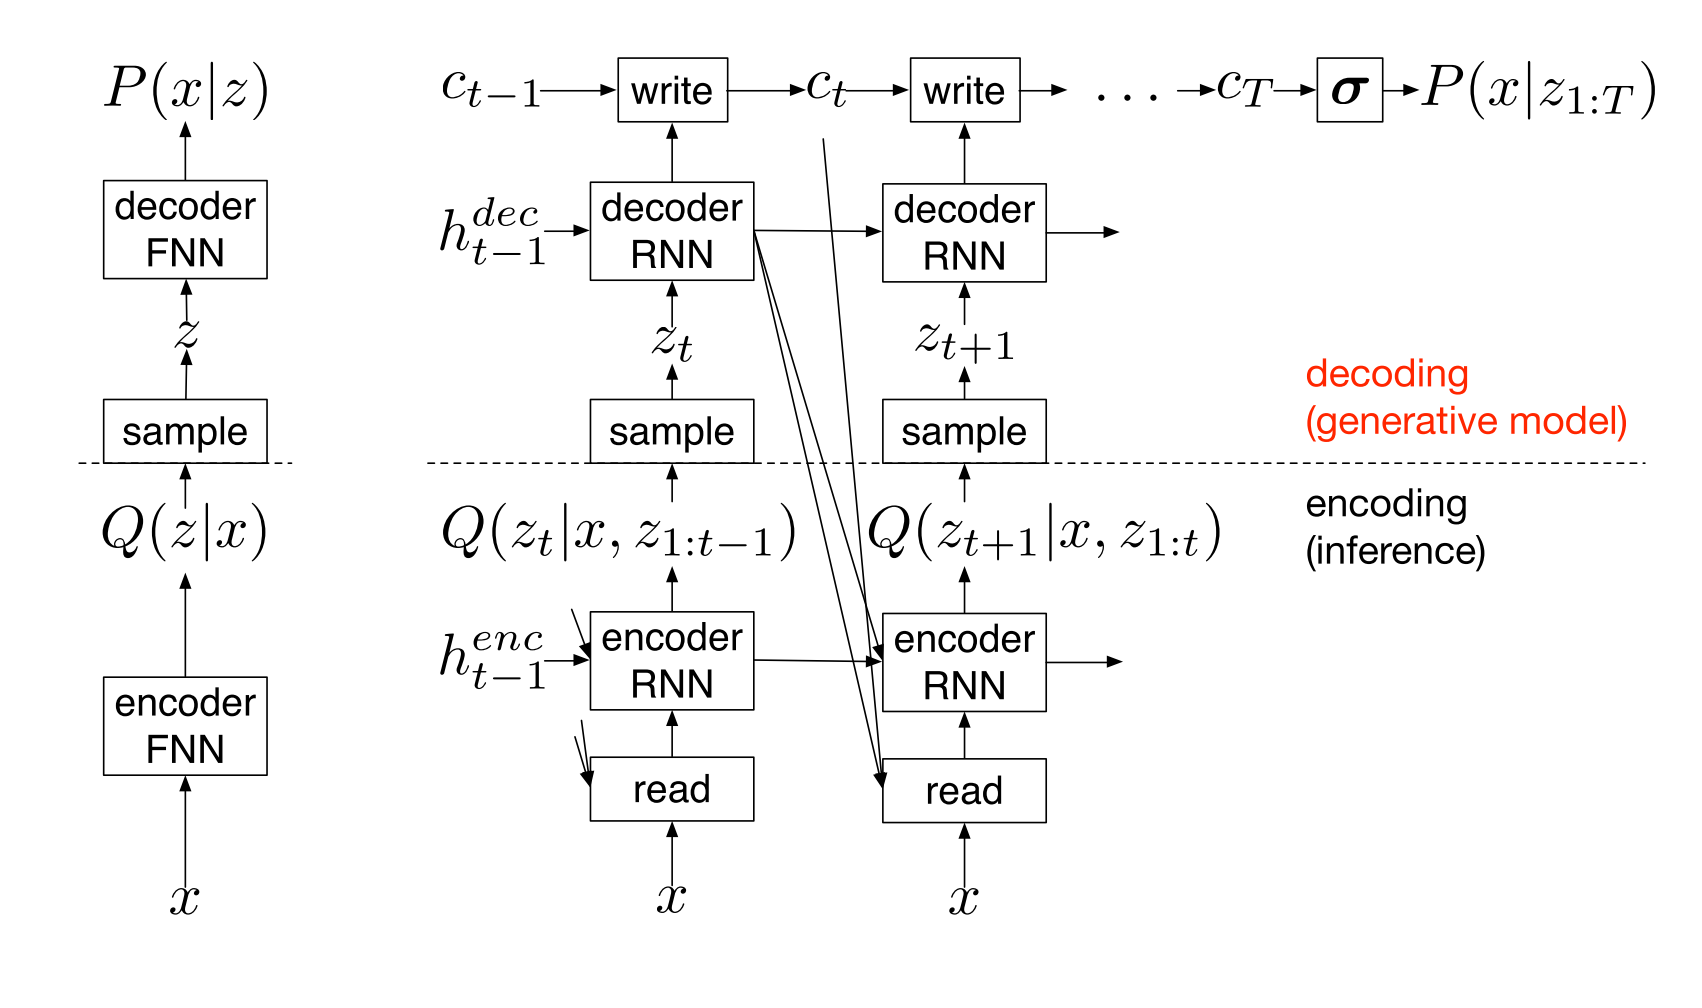
\includegraphics[width=\textwidth]{../figures/draw}
\caption[DRAW network architecture]{\textbf{Left:} an ordinary one\-shot encoder\-decoder network. \textbf{Right:} DRAW network that iteratively constructs the canvas using RNN cells as the encoder/decoder pair. The final output is then iteratively constructed using a series of updates on a canvass, $c_t$. DRAW function read that process the input and feeds this to the encoder which outputs a latent sample $\mathbf{z}_t$. The latent sample in turn acts as input to the decoder part of the network which modifies the canvass using a write function that mirrors the read operation.}\label{fig:draw}
\end{figure}
 
 \subsection{Read and Write functions}

 The read/write functions are paired processing functions that create a sub-sampled representation of the input. The trivial versions of which is just the concatenation of the error image with the input for the read-function and a weight transformation from the decoder state to the output dimension as the write. This pair of functions have not been considered for this work. 

 Instead of the trivial implementations the DRAW network implemented grids of Gaussian filters to extract patches of smoothly varying location and size (\cite{Gregor2015}). To control the patch the authors compute centers,$g_X$ and $g_Y$ , and stride, which controls the size, of a $N \times N$ patch of Gaussian filters over the $H \times W$ input image. The mean location of those filters are computed from the centers, $g_X$ and $g_Y$, and the stride $\delta$. From \citet{Gregor2015} the means at row $i$ and column $j$ are defined as 

 \begin{align}
 \mu_X^i &= g_X + (i - N/2-0.5)\delta, \\
 \mu_Y^j &= g_Y + (j - N/2-0.5)\delta.
 \end{align}

\noindent The attention parameters are computed from a fully connected layer connecting the decoder state to a 4-tuple of floating point numbers i.e

\begin{equation}\label{eq:draw_params}
\tilde{g}_x, \,\tilde{g}_y, \, \log \sigma^2, \, \log \gamma = \text{Dense} (\mathbf{h}_t^{dec}),
\end{equation}

\noindent where $\sigma^2$ is the isotropic variance of the Gaussian filters, and $\gamma$ the multiplicative intensity of the filtering. We parametrize the $\sigma^2$ and $\gamma$ variables in a logarithm to ensure positivity by exponentiating them prior to use. Gregor et. al makes an additional transformation on the centers to ensure that the initial patch roughly covers the entire input image. The transformation is made with respect to the input width, $W$, and height, $H$, giving

\begin{align}
g_x = \frac{W +1 }{2} (\tilde{g}_x +1 ), \\
g_y = \frac{H +1 }{2} (\tilde{g}_y +1 ). \\
\end{align}

\noindent The above equations included terms to compute and scale $\delta$, which we elect to estimate as a constant hyperparameter. As the combination between the number of filters $N$ and $\delta$ determines the size of the input region passed to the encoder. Forcing these glimpses to be equally sized we hypothesize will ensure the comparability of latent samples. Setting $\delta$ as a hyper-parameter was inspired by the work of \citet{Harris2019}.

Given the scaled center we can then compute the filter-banks $F_x \in \mathcal{R}^{N \times W}$ and $F_y \in \mathcal{R}^{N \times H}$

\begin{align}
F_x [i, w] = \frac{1}{Z_x}e^{-\frac{(w - \mu_x^i)^2}{2\sigma^2}},\label{eq:Fx} \\
F_y [j, h] = \frac{1}{Z_y}e^{-\frac{(h - \mu_y^j)^2}{2\sigma^2}},\label{eq:Fy}
\end{align}

\noindent where we denote a point in the input with $(h,\, w)$, and a point in the attention patch with $(i,\, j)$. The filters-banks are multiplied with a normalization constant s.t. $\sum_w F_x[i, w] = 1$, and we define the constant $Z_y$ in the same way. 

Finally we define the read and write functions with attention parameters. The read operation reads a patch from the input and the error image and returns their concatenation to the encoder. To add to the output the write function returns an array that is added to the current canvass $c_t$. From \citet{Gregor2015} the read function is defined as

\begin{equation}\label{eq:read}
\text{read}(\mathbf{x}, \mathbf{\hat{x}}, \mathbf{h}_{t-1}^{dec}) = \gamma[F_y \mathbf{x} F_x^T, F_y \mathbf{\hat{x}} F_x^T].
\end{equation} 

\noindent For the write function we compute a new set of attention parameters which we denote as e.g. $\hat{\gamma}$. Subsequently we compute a dense layer transform from the current decoder state to a matrix $w_t \in \mathcal{R}^{N \times N}$ to ensure the matrix multiplications are sane. The write function is then defined as

\begin{equation}\label{eq:write}
\text{write}(w_t)  = \hat{\gamma} \hat{F}^T_y w_t \hat{F}_x.
\end{equation}

\noindent Notice the transposition order in equation \ref{eq:write} is reversed with respect to the order in equation \ref{eq:read}. 

\subsection{Latent samples and loss}

Optimizing the DRAW algorithm is almost entirely analogous to the procedure for the variational autoencoder. We operate with a divergence over our latent samples and a latent prior, as well as a reconstruction term parameterizing the log evidence. In not so many words we still have a cross entropy loss over the reconstruction and input as well as a divergence term from our latent samples.  

As the DRAW model creates a sequence of latent samples the considerations for the latent loss changes somewhat. In the DRAW algorithm our encoder parametrizes a distribution $q(\mathbf{z}_t | \mathbf{h}_t^{enc})$ which we want to model as being drawn from some prior $p(\mathbf{z}_t)$. As with the variational autoencoder we let the prior be a multivariate isotropic Gaussian. The latent loss, $L_z$, is then a sum over individual divergence terms for each time-step

\begin{equation}\label{eq:draw_latent}
L_z = \sum_t^T D_{KL}(q||p).
\end{equation}

\noindent Given the same prior as for the variational autoencoder we can apply the same derivation of the closed form divergence. Previously we parametrized the latent sample with a mean and standard deviation vector, repeating this procedure the loss becomes 

\begin{equation}\label{eq:draw_kl}
L_z = \frac{1}{2}\sum_t^T(\mu^2_t + \sigma^2_t - \log \sigma_t ^2) - \frac{T}{2}.
\end{equation}

\noindent Similarly the maximum mean discrepancy loss is computed from equation \ref{eq:draw_latent} replacing the Kullback-Leibler divergence with the terms from equation \ref{eq:mmd}.
